\documentclass[letterpaper,11pt]{article}

\usepackage{hyperref}
\usepackage{wrapfig}
\usepackage{pdfpages}
\usepackage[utf8]{inputenc}
\usepackage[spanish,mexico]{babel}
\usepackage{graphicx}
\usepackage{amsmath}
\usepackage{amsthm}
\usepackage{svg}
\usepackage{amsfonts}
\usepackage{subcaption}
\usepackage[margin=1.5cm,
vmargin={1cm,0.3cm},
includefoot]{geometry}
\usepackage{fancyhdr}
\pagestyle{fancy}
\renewcommand{\headrulewidth}{0.4pt}
\renewcommand{\footrulewidth}{0.4pt}


\begin{document}
	\setlength{\unitlength}{1cm}
	\thispagestyle{empty}
	\begin{picture}(19,3)
	\put(-0.5,1.2){\includegraphics[scale=.20]{unam1.png}}
	\put(16,1){\includegraphics[scale=.29]{fciencias1.png}}
	\end{picture}

\begin{center}
\vspace{-114pt}
\textbf{\large Estructuras de Datos}\\
\textbf{ Semestre 2020-2}\\
Prof. Alejandro Hernández Mora\\
Ayud. Pablo Camacho González  \\ 
Ayud. Lab. Luis Manuel Martínez Dámaso   \\
\rule{17cm}{0.3mm}\\
\textbf{Proyecto final}\\
\huge\textbf{Simulador Supermercado}\\[0.1cm]
\normalsize Kevin Ariel Merino Peña\footnote{317031326}\\
Armando Abraham Aquino Chapa\footnote{317058163}\\
\rule{17cm}{0.3mm}
\end{center}
%\vspace{-10pt}
%\begin{flushright}
%\vspace{-3pt}
%end{flushright}
\section*{Modelo del programa:}
\begin{figure}[htb]
	\centering
	\includegraphics[scale=.23]{Simbologia.png}
	\caption{ Simbología para los diagramas de clases}
\end{figure}
A continuación se presentará una breve descripción del modelo del programa para la simulación del comportamiento de un supermercado con sus respectivos diagramas de clases.\\

\textbf{Main: }Contiene nuestro método principal que permite cumplir con el encapsulamiento y comportamiento del programa.
\begin{figure}[htb]
	\centering
	\includegraphics[scale=.27]{main_diagram.png}
\end{figure}

\textbf{Package UImenu: } Contiene nuestra clase \textit{Menu} dónde modelamos la interacción con la usuaria. Entre sus métodos principales se encuentran:

\begin{itemize}
	\item \textit{mainMenu: } Cómo su nombre lo indica se encarga de proveer dos opciones principales; "Modo Usuario", "Modo Administrativo" y por supuesto una opción para salir.
\end{itemize}
\begin{itemize}
	\item \textit{adminMenu:} Para uso administrativo del supermercado, en el cual podemos agregar, resurtir y ver el inventario de productos del mismo.
\end{itemize}
\begin{itemize}
	\item \textit{userMenu: } Aquí encontramos las funciones de las que podrá hacer uso cualquier persona, como hacer una simulación automática del supermercado, ó una simulación más personalizada ingresando el número de cajas rápidas y normales.
\end{itemize}
\begin{itemize}
	\item \textit{execPlot: } Se crean gráficas a partir del resultado de las simulaciones del supermercado para apreciar el comportamiento y rendimiento de las cajas del mismo para estudios posteriores.
\end{itemize}
\begin{figure}[htb]
	\centering
	\includegraphics[scale=.24]{menu_diagram.png}
\end{figure}

\textbf{Package util: } En este paquete encontramos diversas clases, entre las cuales destacan las estructuras de datos utilizadas para modelar el supermercado y todo lo que lo engloba. Las estructuras de datos utilizadas son: \textit{Árbol Binario, de Búsqueda, Árbol AVL, Cola, Heap, Lista, Pila.}\\

También encontramos una clase llamada \textit{Utilities}, la cuál tiene la funcionalidad de contar con métodos auxiliares de la clase \textit{Menu } para que el programa sea persistente.\\
Por último encontramos dos clases llamadas \textit{Item, ItemBuilder} que generan productos aleatorios para el supermercado.\\
A continuación la representación en diagrama de clases.
\newpage
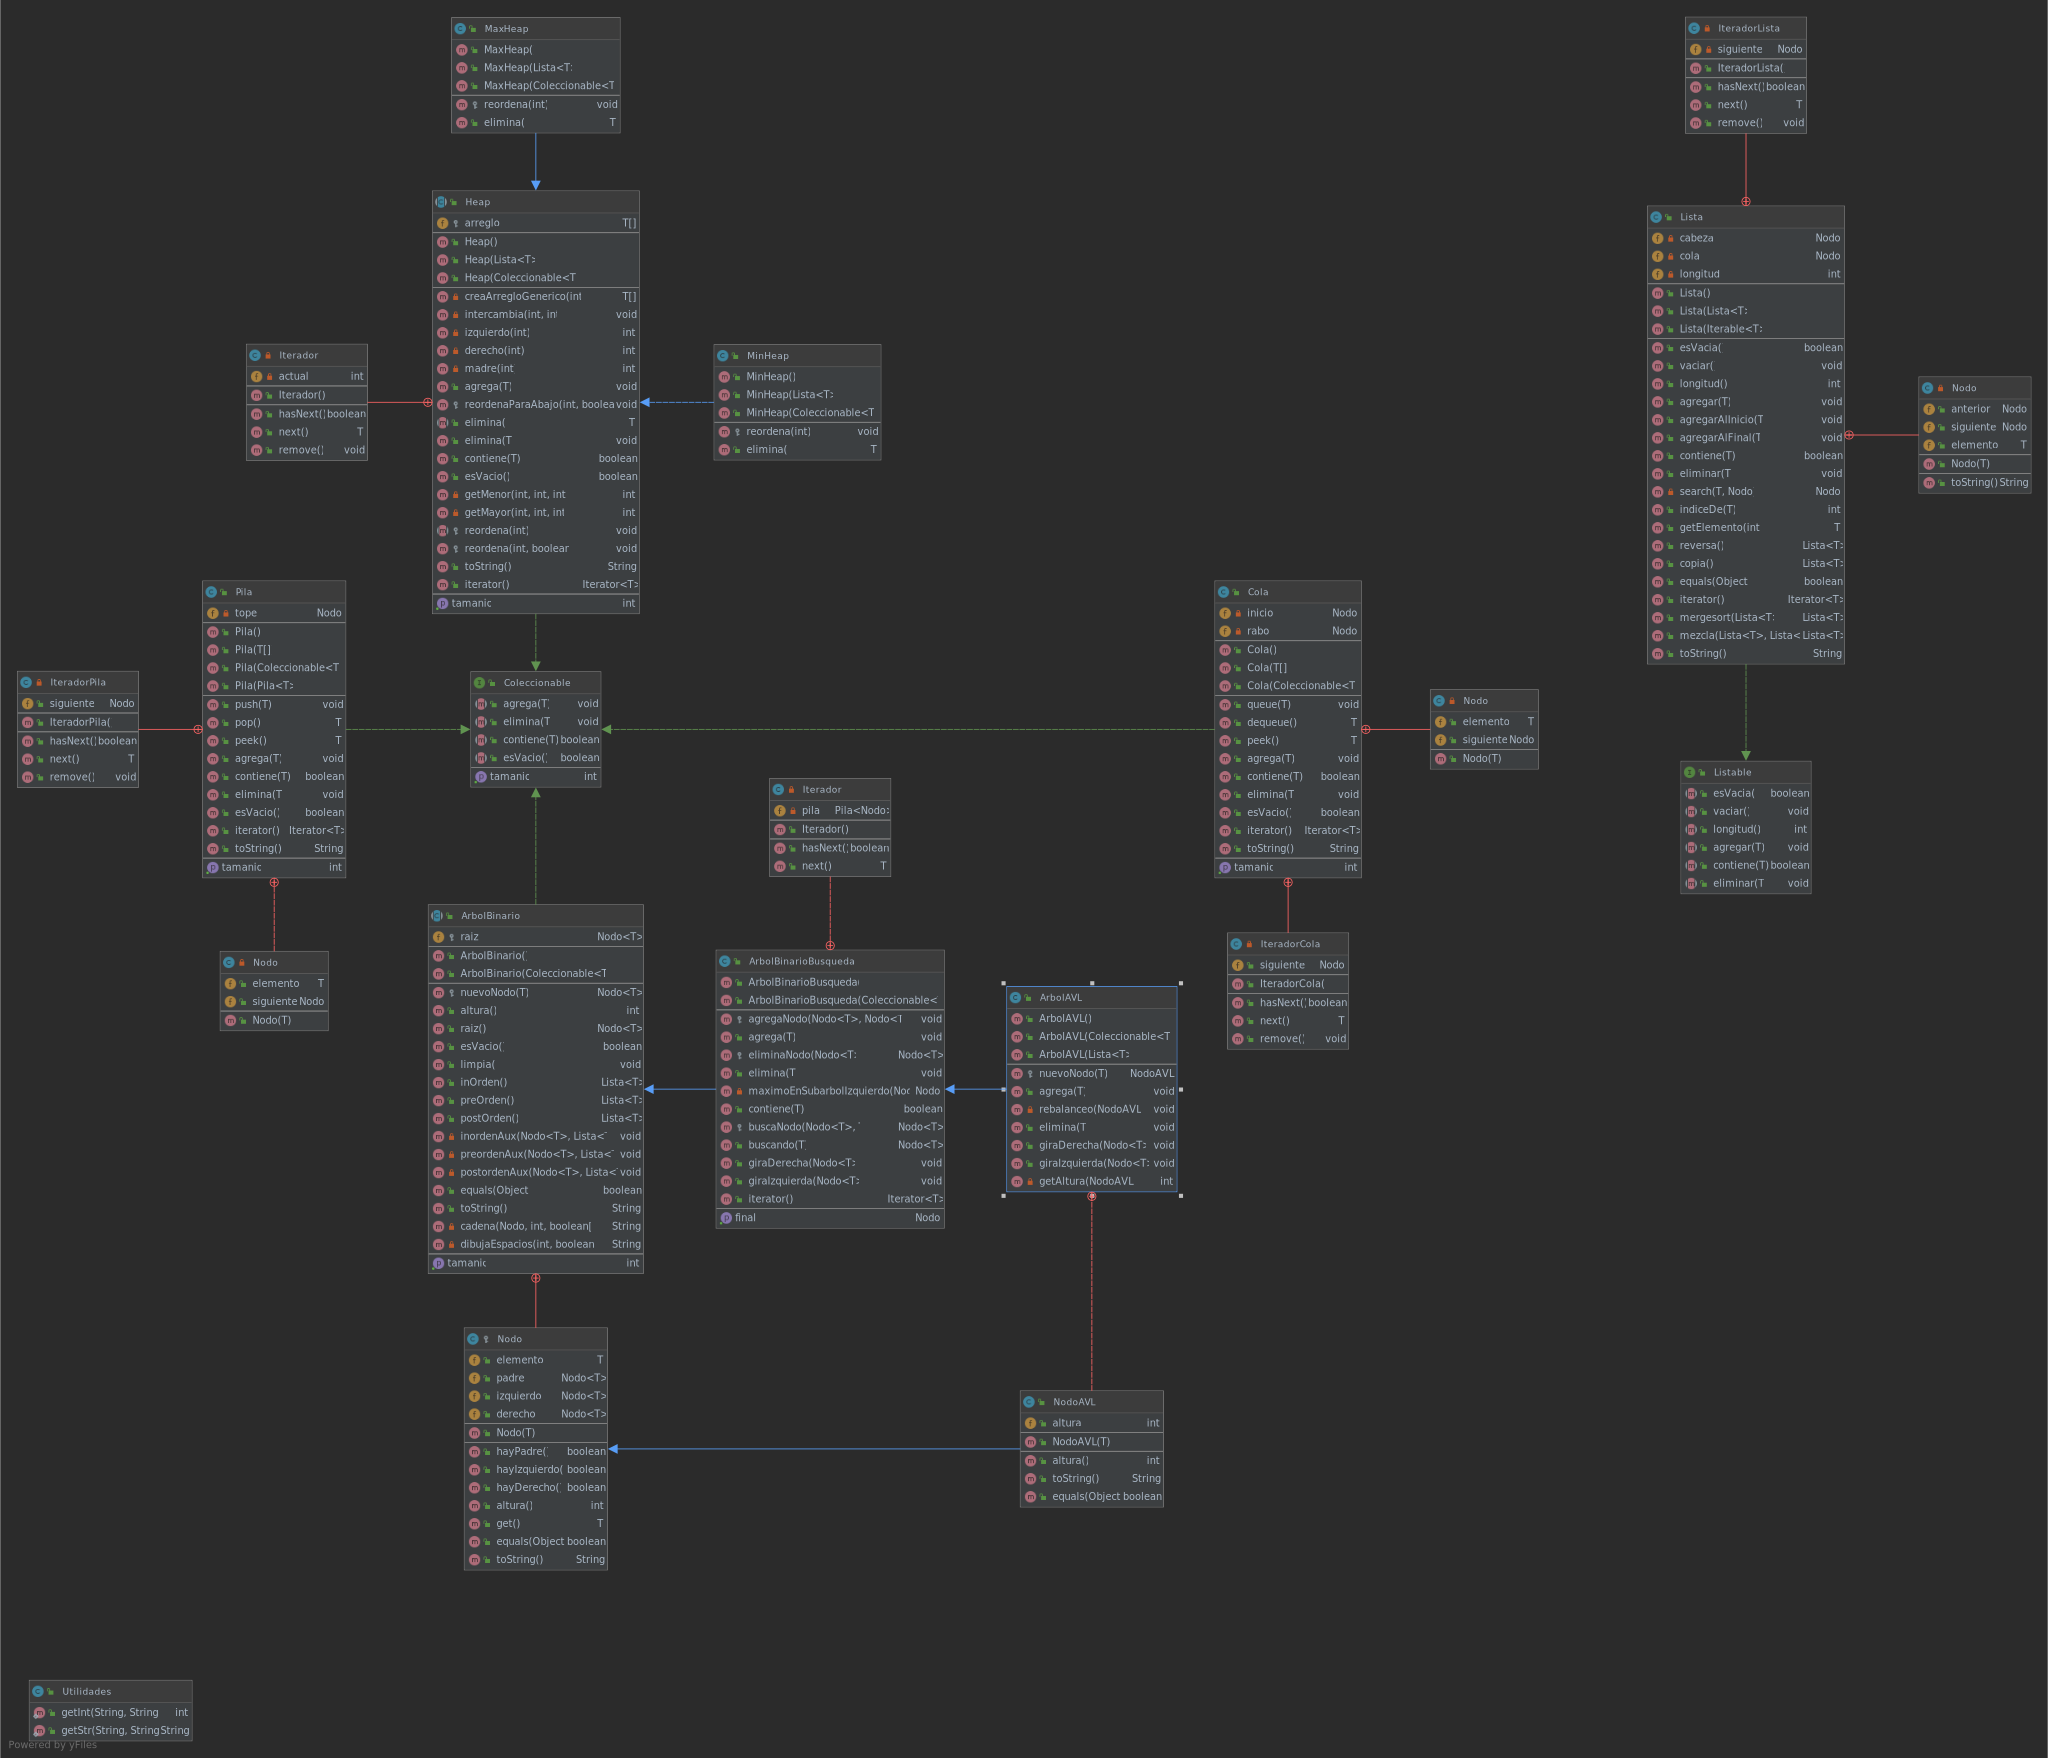
\includepdf[pages=-]{util}
\textbf{Package sim: } Este paquete contiene las clases necesarias que se encargan de gestionar la simulación del supermercado a través de hilos.
\begin{itemize}
	\item \textit{enterClient: } Simula el estado de un cliente en el supermercado, desde su ingreso a éste, formarse en alguna caja y pagar sus productos.
\end{itemize}
\begin{itemize}
	\item \textit{Simulation: } Engloba y ejecuta todos los aspectos necesarios para el comportamiento del supermercado. Un método a destacar es \textit{getReports} el cuál crea diversos directorios dónde se almacena el estado del supermercado después de las simulaciones, es decir, que productos tienen pocas existencias, los tickets generados de las diversas compras de los clientes, etc.
\end{itemize}
\begin{figure}[htb]
	\centering
	\includegraphics[scale=.33]{sim_diagram.png}
\end{figure}
\textbf{Package market: }
\begin{itemize}
	\item \textbf{Package admin: } Aquí se encuentran las clases para modelar los objetos que componen a un supermercado, tales como sus cajas (hay dos tipos: normal y rápida), sus productos (los cuales poseen un ID generado aleatoriamente, unidades en el inventario, nombre, precio) y un almacén dónde podemos consultar el inventario, modificar, ver los productos ue contiene, etc. 
\end{itemize}
\newpage
\includepdf[pages=-]{admin}
Por último tenemos la clase \textit{Supermaket } que permite relacionar del paquete \textit{admin} y le otorga una estructura al supermercado.
\begin{figure}[htb]
	\centering
	\includegraphics[scale=.31]{supermarket_diagram.png}
\end{figure}
\section*{Reporte de resultados:}
Para determinar cuál es el número óptimo de cajas rápidas que deben operar en el supermercado, haremos uso de las gráficas producidas automáticamente a partir de las simulaciones generadas por el proyecto que se nos solicitó hacer para la resolución del problema mencionado.\\
Antes del análisis y presentación del resultado consideremos los siguientes aspectos.
\begin{itemize}
	\item \textit{Tipo.} Mostraremos dos tipos de gráficas; histograma y gráfica de puntos.\\
	La primera proporciona la información de cuántos clientes rápidos y cuántos clientes normales fueron atendidos en el supermercado, para así poder apreciar/estimar la volatilidad de los mismos durante cada simulación.\\
	Por otra parte, la de puntos provee información de la eficiencia por número de cajas rápidas abiertas en cuánto al promedio del tiempo de espera de los clientes.
\end{itemize}
\begin{itemize}
	\item \textit{Escala.} Cada gráfica presentada toma en cuenta un total de catorce simulaciones que representan dos semanas de funcionamiento del supermercado, esto con el fin de que por cada día, una nueva caja rápida entre en operaciones, es decir, en el día uno sólo habrá una caja rápida, y en el día catorce habrá catorce cajas rápidas (recordar que el supermercado cuenta con quince cajas). A excepción de la gráfica de puntos (será mostrada más adelante), la cuál toma en cuenta un total cincuenta y seis simulaciones (cuatro simulaciones distintas por caja rápida).
\end{itemize}
\textbf{Análisis:}\\
En una primer simulación, mediante el siguiente histograma podemos apreciar que cuando se encuentran abiertas tres cajas rápidas en operación (día tres), es el día en que se produce una mayor fluctuación entre clientes normales y rápidos.\\ Por otra parte, cuando se encuentran trece cajas rápidas abiertas notamos un balance entre ambos tipos de clientes. Siendo con dos, seis y siete cajas rápidas abiertas con más clientes atendidos (64,62, 62 respectivamente).
\begin{figure}[htb]
	\centering
	\includegraphics[scale=.20]{Barras1.jpeg}
	\caption{Primer histograma}
\end{figure}\\
En una segunda simulación percibimos que la mayor fluctuación entre clientes es con cinco cajas rápidas(día cinco), dónde aproximadamente se atendieron a cincuenta y cuatro clientes.\\ Asimismo, en las cajas tres y cuatro con alrededor de cincuenta y ocho clientes es cuando hay un mayor equilibrio. Siendo las cajas seis, siete, tres, cuatro, ocho con más clientes atendidos (57, 56, 56, 56, 56 respectivamente)
\begin{figure}[htb]
	\centering
	\includegraphics[scale=.20]{Barras2.jpeg}
	\caption{Segundo histograma}	
\end{figure}\\
Una última simulación indica que en la caja diez (décimo día) ocurre la mayor fluctuación, y en la caja cuatro y siete tenemos el mejor balance entre clientes.\\Siendo las cajas tres y doce con más clientes atendidos (ambos con 56), seguidos por los cajas siete siete, cuatro, once, tres (todas con 55).\\

\begin{figure}[htb]
	\centering  
	\includegraphics[scale=.20]{Barras4.jpeg} 
	\caption{Tercer histograma} 
\end{figure}

Entonces, de los histogramas presentados anteriormente, podemos inferir que los días seis y siete fueron los días que más clientes atendieron, debido a que en todas las simulaciones presentadas a través de la gráfica, éstas cajas fueron las que obtuvieron los mejores resultados.\\Por último analicemos la gráfica de puntos para determinar si se deben abrir seis ó siete cajas rápidas en el supermercado.
\begin{figure}[htb]	
	\centering
	\includegraphics[scale=.21]{PuntosMultiple.png}
	\caption{De puntos}
\end{figure}\\

De igual forma, en esta gráfica podemos apreciar que el eje \textit{x} está conformado por el número de cajas rápidas abiertas por simulación, mientras que el eje \textit{y} representa el promedio de tiempo (en milisegundos) de espera de los clientes.\\Primero veamos que las cajas con más promedio de tiempo de espera son las cajas uno (acotada inferiormente por 410 ms y superiormente por 560 ms) y la caja diez (acotada inferiormente por 430 ms y superiormente por más de 580 ms). Por otro lado la caja con el mejor promedio de tiempo de espera es la ocho (acotada inferiormente por 450 ms y superiormente por 490 ms).\\Ahora bien, ya hemos determinado que las cajas seis y siete tuvieron el mejor desempeño en los histogramas, entonces hay que analizar cuál de esas dos cajas está mejor acotada en cuánto al promedio de tiempo de espera. Esto es fácil de ver, ya que la caja seis se encuentra acotada inferiormente por 450 ms y superiormente por 550 ms, mientras que la cota inferior de la caja siete es de 460 ms, y su cota superior es de 500 ms.\\ Por lo tanto el número de cajas rápidas que han tenido el mejor rendimiento en las gráficas son siete.\\

\textbf{Conclusión}\\

Por el análisis descrito anteriormente, y su representación en histogramas y gráficas de puntos, concluimos que el número óptimo de cajas rápidas que deben operar el supermercado son siete cajas.\qed\\

\href{https://drive.google.com/drive/folders/1razQHfkaCekMu2o-5wroSP_411UXS1QN?usp=sharing}{Pulsa aquí para acceder a los recursos empleados para la elaboración del reporte}
 

\end{document}
